\documentclass{article}

% Basic packages
\usepackage[a4paper,margin=1.5cm]{geometry}
\usepackage{amsmath, amssymb}
\usepackage{graphicx}
\usepackage{float}
\usepackage{booktabs}
\usepackage{array}
\usepackage{tabularx}
\usepackage{xcolor}
\usepackage{pifont}
\usepackage{multirow}
\usepackage{setspace}

\usepackage[backend=biber, style=numeric, citestyle=numeric]{biblatex}
\addbibresource{references.bib}
\newcommand{\cmark}{\ding{51}}%
\newcommand{\xmark}{\ding{55}}%


\title{Thesis Draft}
\author{Simone Pagliuca}

\begin{document}
\raggedright
\doublespacing

% TEMPORARY
\textcolor{orange}{Citation of \cite{PLACEHOLDER} are placeholders for facts or data that need citation.}
% Introduction to the study, context and motivation to support it
% Definition of the research problem and questions
\section*{Introduction}
\label{sec:introduction}
\section*{A brief History of Nuclear Power, from its origins to present day}
The 1930s and 1940s witnessed unprecedented acceleration in nuclear science. Following James Chadwick's 1932 discovery of the neutron \cite{PLACEHOLDER}, Otto Hahn and Fritz Strassmann demonstrated nuclear fission in 1938 by producing barium through uranium neutron bombardment \cite{PLACEHOLDER}. This breakthrough enabled Enrico Fermi's team to construct Chicago Pile-1 in 1942 - the first artificial nuclear reactor capable of sustaining and controlling a chain reaction \cite{PLACEHOLDER} - just four years after the fission discovery.

While initial advancements were primarily motivated by military applications during World War II, culminating in the atomic bombings of Hiroshima (August 6, 1945) and Nagasaki (August 9, 1945), the scientific community quickly recognized nuclear technology's peaceful potential. President Eisenhower's 1953 "Atoms for Peace" address to the United Nations \cite{PLACEHOLDER} established the foundation for international nuclear cooperation, leading to the 1957 creation of both the International Atomic Energy Agency (IAEA) and the European Atomic Energy Community (EURATOM). These institutions were tasked with promoting peaceful nuclear applications while serving as independent authorities for safety regulation and non-proliferation oversight.

The 1950s and 1960s marked a period of rapid nuclear reactor development, driven by dual civilian and military imperatives. This era saw several key milestones in nuclear power generation: the Experimental Breeder Reactor I (EBR-I) in Idaho (USA) first produced electricity in 1951 (powering four light bulbs) \cite{PLACEHOLDER}, followed by the Obninsk Nuclear Power Plant (USSR) in 1954, which became the first to feed approximately 5 MWe into a local grid \cite{PLACEHOLDER}. The world's first commercial-scale nuclear power station, Calder Hall-1 (UK), began operation in 1956, connecting to the national grid with an initial capacity of 50 MWe \cite{PLACEHOLDER}.

Parallel technological diversification occurred during this period. The United Kingdom developed gas-cooled Magnox reactors, optimized for both electricity production and plutonium generation. Concurrently, the Soviet Union initiated development of the graphite-moderated, water-cooled RBMK design through experimental work at Obninsk. Canada's nuclear program focused on pressurized heavy water reactor (PHWR) technology, culminating in the 1962 Rolphton demonstration reactor and the first commercial CANDU reactor at Douglas Point in 1968 \cite{PLACEHOLDER}.

In reactor cooling technologies, the United States pioneered multiple approaches: the EBR-I employed liquid metal (NaK) cooling, while the naval propulsion program led to light water reactor (LWR) development with the 1954 launch of USS Nautilus. By 1957, both Boiling Water Reactor (BWR) and Pressurized Water Reactor (PWR) designs were adapted for civilian applications, with the Shippingport Reactor (Pennsylvania) becoming the first full-scale civilian PWR connected to the grid. The Soviet VVER ("Water-Water Energetic Reactor") program advanced simultaneously, deploying the 210 MWe VVER-210 at Novovoronezh Nuclear Power Plant in 1964 \cite{PLACEHOLDER}.

The 1960s and 1970s witnessed significant global expansion of nuclear power generation. During this period, numerous countries commissioned their first nuclear reactors: Argentina (Atucha-1, 1974), Armenia (Armenian-1, 1976), Belgium (BR-3, 1962), Bulgaria (1974), Italy (Latina, 1963), Japan (1963), Sweden (1964), Switzerland (1969), and Slovakia (1972) \cite{PLACEHOLDER}.

The 1973 oil crisis accelerated nuclear adoption as an energy security strategy. France implemented the Messmer Plan, an ambitious program that resulted in the construction of 43 reactors between 1977 and 1986 \cite{PLACEHOLDER}. Similarly, Japan significantly expanded its nuclear capacity to reduce dependence on imported oil, establishing nuclear energy as a cornerstone of its national energy strategy \cite{PLACEHOLDER}.

The nuclear expansion continued through the 1980s until the 1986 Chernobyl disaster, which constituted a critical inflection point for global nuclear development. The accident prompted widespread safety reviews and regulatory updates, significantly slowing deployment rates \cite{PLACEHOLDER}. Public opposition intensified particularly in Western Europe, leading several countries to halt or reduce their nuclear programs. Italy's 1987 referendum resulted in the complete phase-out of nuclear power, while other European nations experienced similar setbacks \cite{PLACEHOLDER}.

By the 1990s, multiple countries had suspended nuclear deployment entirely, including Germany and Switzerland. France, previously the most active builder, connected only 10 reactors between 1990-1999, while the United States and United Kingdom deployed 4 and 1 reactors respectively during the same period \cite{PLACEHOLDER}. Italy completed its nuclear phase-out by 1990 with the permanent shutdown of all operating reactors. Following the post-Soviet economic transition, Russia resumed its nuclear program and has since maintained continuous expansion of its reactor fleet \cite{PLACEHOLDER}.

A nuclear renaissance emerged in the early 2000s, driven by concerns over climate change, energy security, and rising fossil fuel prices. This period saw the development of advanced reactor designs including the European Pressurized Reactor (EPR) and AP1000 \cite{PLACEHOLDER}. However, the 2011 Fukushima Daiichi accident constituted another significant setback for nuclear expansion in Western nations. Projects faced substantial delays, cost overruns, and public opposition, with France's Flamanville-3 EPR serving as a particularly illustrative case: experiencing budget increases to eight times original estimates and construction timelines tripled from initial projections \cite{PLACEHOLDER}. Germany accelerated its nuclear phase-out policy, while Italy reaffirmed its anti-nuclear position through a popular referendum \cite{PLACEHOLDER}.

Contrastingly, Eastern nations pursued markedly different nuclear trajectories. China, having initiated its nuclear program in the 1990s with Qinshan-1 (connected in 1991), has since maintained aggressive expansion. Over the past three decades, China has brought 56 additional reactors online and currently has 29 under construction, positioning itself to surpass both France and the United States in total reactor capacity within coming decades \cite{PLACEHOLDER}. This expansion reflects a strategic commitment to nuclear energy as part of China's broader energy and climate objectives.

The COVID-19 pandemic in 2020 exposed critical vulnerabilities in global economic systems, while Russia's 2022 invasion of Ukraine further revealed Europe's energy security dependencies \cite{PLACEHOLDER}. Concurrently, decarbonization imperatives to combat climate change have prompted Western nations to reconsider nuclear energy's dual role: providing low-carbon, reliable baseload power while enhancing energy independence and system resilience \cite{EU2050ClimateStrategy}.

This strategic reassessment is evident in recent policy initiatives. The European Union's classification of nuclear power as a sustainable investment under its taxonomy for climate mitigation \cite{EUTaxonomy}, alongside programs like the U.S. Department of Energy's Advanced Reactor Demonstration Program \cite{PLACEHOLDER}, demonstrates renewed interest in nuclear technologies. The European energy sector is consequently undergoing a significant transformation, balancing decarbonization targets with energy security requirements through diversified generation portfolios that include advanced nuclear solutions \cite{EU2050ClimateStrategy}.

While the political decision to include nuclear power is fundamentally a strategic choice, selecting specific reactor designs involves complex trade-offs across technical, economic, regulatory, social, environmental, and geopolitical dimensions \cite{PLACEHOLDER}. National energy needs vary significantly: some countries require large baseload capacity to reduce import dependence, while others prioritize smaller, more flexible solutions to integrate with existing renewable systems \cite{PLACEHOLDER}.

The current nuclear landscape presents particular challenges for decision-makers, offering both established Generation III+ designs and emerging Small Modular Reactors (SMRs) as potential options. Given that nuclear commitments represent decade-long investments with 60-year operational lifespans \cite{PLACEHOLDER} and significant financial implications, and considering the multiple influencing factors like grid infrastructure, public acceptance, and supply chain considerations, policymakers require structured decision-support tools to evaluate these complex trade-offs. This study therefore employs Multi-Criteria Decision Analysis (MCDA), specifically the Multi-Attribute Value Theory (MAVT) approach, presented in the following paragraphs.

\subsection*{MCDA and MAVT as a Decision Support Tool}
Multi-Criteria Decision Analysis (MCDA) provides a structured, transparent framework for addressing complex decision problems where trade-offs between competing objectives are inevitable. Common to any decision making process is a systematic process that involves: defining the decision problem, identifying relevant objectives, establishing alternative decision options, and quantifying the performance of each option against these objectives. \\

Among these methods, Multi-Attribute Value Theory (MAVT) employs a hierarchical objective structure and value functions to convert both qualitative and quantitative data into comparable units. By assigning importance weights to each attribute, MAVT aggregates these measurements into a single composite score for each option. This approach is particularly effective for ranking alternatives and providing decision-makers with a comprehensive comparison of available options. \\

\textcolor{orange}{how much more do I have to explain here? I guess that I will explain the way we apply weights when we do it, the way swing elicitation works when we apply it etc etc...}
\section{A brief History of Nuclear Power}
\subsection{Origins}
The 1930s and 1940s witnessed rapid advancement in nuclear science. In 1932 James Chadwick discovered of the neutron \cite{Chadwick_Neutron_1932} and a year later Leo Szilard hypothesized fission chain reactions. In 1938, Otto Hahn and Fritz Strassmann produced barium by bombarding uranium with neutrons, demonstrating nuclear fission \cite{Hahn_Strassmann_1939}. Further advancements like the first controlled nuclear chain reaction in the Chicago Pile-1 achived by Enrico Fermi's team in 1942, were speed up by World War II as part of the Manhattan Project which lead to the atomic bombings of Hiroshima (6 August 1945) and Nagasaki (9 August 1945). The recognition among the scientific community of the peaceful potential of nuclear technology lead to the famous speech "Atoms for Peace" by USA President Eisenhower in 1953 to the United Nations \cite{Eisenhower_Atoms_for_Peace_1953} which established the foundation for international nuclear cooperation. The International Atomic Energy Agency (IAEA) and the European Atomic Energy Community (EURATOM) were established 4 years after, in 1957, and were tasked with promoting peaceful nuclear applications while serving as independent authorities for safety regulation and non-proliferation oversight.

\subsection{Generation I}
The 1950s marked the emergence of numerous reactor designs, driven by both civilian energy needs and military applications. These early models, now classified as Generation I reactors, represent the first prototypes of nuclear power at utility scale. The Experimental Breeder Reactor I (EBR-I) in Idaho (USA), which first generated electricity in 1951 (powering four light bulbs). The Obninsk Nuclear Power Plant (USSR), which in 1954 became the first to feed approximately 5 MWe into a local power grid. Calder Hall-1 (UK), the world's first commercial-scale nuclear power station, which began operation in 1956 with a 50 MWe capacity connected to the national grid

The United States pioneered light water reactor (LWR) technology through two distinct designs: the Boiling Water Reactor (BWR) and the Pressurized Water Reactor (PWR) which was originally developed for naval propulsion. The first commercial implementations of the BWR was the Dresden-I (1960) and for the PWR the Shippingport Atomic Power Station (1957) \cite{IAEA_PRIS_2025}. Concurrently, the USSR developed its own pressurized water technology, the VVER ("Water-Water Energetic Reactor"), featuring design characteristics that persist in modern variants.

This period also witnessed significant technological diversification as other nations developed their own reactor designs. The United Kingdom advanced gas-cooled Magnox reactors, optimized for dual electricity and plutonium production. The Soviet Union initiated development of the graphite-moderated, water-cooled RBMK design, while Canada's nuclear program focused on pressurized heavy water reactor (PHWR) technology, culminating in the first commercial CANDU reactor at Douglas Point in 1968 \cite{IAEA_PRIS_2025}.


\subsection{Generation II}
Between the 60s and 70s Generation II reactors were deployed, taking advantage of the experience from the previous run, these reactors are not anymore considered experiments or prototypes but fully commercial power plants. In these decades numerous countries commissioned their first nuclear reactors: Belgium (1962), Italy (1963), Japan (1963), Sweden (1964), Switzerland (1969), Slovakia (1972), Argentina (1974), Bulgaria (1974) and Armenia (1976) \cite{IAEA_PRIS_2025}. Following the 1973 oil crisis, the deployment of nuclear power plants was accelerated in some countries as an energy security strategy. Most notably France implemented the Messmer Plan, named after the Prime Minister at the time, to greatly expand the nuclear plant fleet \cite{FundingUniverse_EDF_History_2025}. 

Nuclear expansion continued through the 1980s until 1986. As news from the Chernobyl disaster came to western countries, fear of the potential risks of nuclear power intensified. The public opposition grew significantly so that, even if safety and regulatory updates were implemented, several countries decided to slow down, reduce or halt their nuclear programs althogether, such was the case of Italy after the results of the 1987 referendum, which resulted in a complete phase-out of nuclear power \cite{MinisteroInterno_Referendum_1987, IAEA_PRIS_2025}. 

By the 1990s, multiple western countries had suspended nuclear deployment entirely, including Germany and Switzerland. France, previously the most active builder, connected 10 reactors between 1990-1999, while the United States and United Kingdom only deployed 4 and 1 reactors respectively during the same period. Italy completed its nuclear phase-out by 1990 with the permanent shutdown of all operating reactors \cite{IAEA_PRIS_2025}. 

Contrastingly, Eastern nations pursued an opposite trajectory. Following the post-Soviet economic transition, Russia resumed its nuclear program and has since continued expansion of its reactor fleet \cite{IAEA_PRIS_2025}. China initiated its nuclear program in the 1990s with Qinshan-1 (connected in 1991) and has since maintained aggressive expansion. Over the past three decades, China has brought 56 additional reactors online and currently has 29 under construction, positioning itself to surpass both France and the United States in total reactor capacity within the coming decade \cite{IAEA_PRIS_2025}.

\subsection{Generation III}
As a result of the regulatory safety improvements, a stabilized choice of technology with LWRs settling as the to go choice all over the world and even larger capacities, Generation III reactor started to be developed in the 90s.

The improvement of these designs was fueled in the early 2000s by concerns over climate change, energy security, and rising fossil fuel prices, leading to Generation III+ reactors, such as the European Pressurized Reactor (EPR) or the US AP-1000 which improve safety and reliability in a consolidated plant layout. However after the 2011 Fukushima Daiichi accident Western nations experienced a significant setback: Germany accelerated its nuclear phase-out policy, while Italy reaffirmed its anti-nuclear position through a popular referendum \cite{MinisteroInterno_Referendum_2011}. In the following years projects faced substantial delays, cost overruns, and public opposition, with France's Flamanville-3 EPR serving as a particularly illustrative case experiencing budget increases to more then four times original estimates and construction timelines tripled from initial projections \cite{nea2020unlocking}.

\subsection{Generation IV}
From the late 2000s to nowadays, new nuclear commissioning projects can be classified as "Mega Projects", such term is used to refer to very large committments where economies of scale tend to fail due to the complexity of the task at hand, resulting in massive delays and cost overruns, well known examples of Mega Projects are Suez and Panama Canals, the Sydeny Opera House or the development of the Concorde Supersonic Aeroplane \cite{Flyvbjerg2014, BROOKES201557}. 

To counter this phenomena, the nuclear industry is developing Small Modular Reactors (SMRs) which are part of Generation IV reactors. SMRs are smaller, standardized reactors that can be built mostly off site to take advantage of economies of multiples. Some SMR designs are based on novelty technologies while others take advantage of well known water-based designs. 

Other generation IV reactors are being design to tackle on other aspects of nuclear power such as waste minimization or higher efficiencies. Manly by emplying different means of cooling to exploit neutrons at higher energies (fast neutrons), or by using thorium instead of uranium as fuel or even using direct gas based cycles to increase thermal efficiency.

\subsection{Current European Landscape}
This historical overview demonstrates the complexity behind the decision to adopt nuclear power which since it's beginning has been a matter of strategic geopolitical and historical consideration rather than purely technical or economic factors. So for starters we observed the current situation and consideration of nuclear energy in europe:

In 2020, the COVID-19 pandemic exposed vulnerabilities in global economic systems and Russia's invasion of Ukraine in 2022 further revealed Europe's energy dependencies \cite{BRODNY2023121443, Sterling_European_Energy_Import_2025, EPRS_Energy_2023}. At the same time, decarbonization goals to combat climate change have prompted Western nations to reconsider nuclear energy as a valid power source able to provide low-carbon, reliable power while enhancing energy independence and system resilience \cite{EU2050ClimateStrategy}.

This strategic reassessment of nuclear is evident in recent policy initiatives. The European Union's classification of nuclear power as a sustainable investment under its taxonomy for climate mitigation \cite{EUTaxonomy}, alongside programs like the European Industrial Alliance on \glspl{smr} are a clear indicator of the renewed interest in nuclear technologies.

\section{Decision Support}
Nuclear energy decisions extend far beyond technical and economic considerations, inevitably encompassing social and political dimensions. This inherent complexity requires \glspl{dm} to evaluate numerous trade-offs across competing objectives in pursuit of balanced, optimal solutions. The systematic process of navigating trade-offs to arrive at informed choices constitutes the fundamental challenge of decision-making.

The decision making process begins by identifying the decision problem and the possible solutions to such problem. Then, there are several ways to approach the decision. The most common approach to decision making, which is encountered by anyone daily in day to day life, is to look at the possible solutions or "alternatives", compare positive and negative outcomes based on own preferences and find the best, or less worst, between them.

For more complex situations such as regarding energy systems, analytical frameworks, usually referred to as \gls{dss}, have been developed to support \glspl{dm}. In the realm of business and management, for example, \glspl{dss} are usually softwares that collect and organize data, communications or knowledge to provide support by data analyses, visualization or by applying models. \cite{Power2023}.

This study focuses on nuclear energy related decision making processes. The literature review reveals that \gls{mcda} methods predominate in energy decision support research. This observation aligns with findings from Seran et al. (2025), whose comprehensive analysis of renewable energy studies demonstrated that the vast majority employed \gls{mcda} methodologies \cite{SERAN2025100044}.

\gls{mcda} systematically evaluates alternative solutions by decomposing decision problems into distinct criteria representing either the consequences of each alternative or their distinguishing characteristics \cite{ROY1990324}. This criterion-based approach offers two primary advantages: first, it enables the structured analysis of complex problems involving many criteria; second, it reveals preference patterns from different perspectives, which becomes particularly valuable when multiple stakeholders are involved. The method's transparency allows decision-makers to identify the most critical aspects of each alternative in relation to specific stakeholder preferences.

While there exists many \gls{mcda} methodologies (see Greco et Al. 2016 \cite{Köksalan2016} and Cinelli et al. 2020 \cite{CINELLI2020102261}) their common ground is to model the decision problem considering all availble information on it, considering trade-offs and then allowing to choose between alternatives \cite{HAAG2022105361}. \gls{mcda} can be used for solving different decision problems:
\begin{itemize}
\item Choice: Selecting the most preferred alternative(s) from a large pool of options.
\item Sorting: Classifying alternatives into predefined categories.
\item Ranking: Ordering all alternatives from most to least preferred.
\item Scoring: Ranking alternatives while also quantifying the differences between them.
\end{itemize}

A fundamental distinction exists between American and European \gls{mcda} methodologies. American-developed approaches, including the \gls{ahp} and \gls{mavt}, were born on the basis of the compensatory principle, emphasizing trade-off dynamics where a disadvantage in one criterion can be offset by an advantage in another.

In contrast, European researchers developed non-compensatory methods based on the outranking principle, such as ELECTRE and PROMETHEE. These methods establish preferences through binary outranking relationships between alternatives (e.g., "alternative A1 is preferred to A2 on regard to criterion C1") and may incorporate veto conditions between criteria. Unlike compensatory approaches, outranking methods focus on meeting requirements rather than optimizing trade-offs \cite{HUANG2026103438, Köksalan2016}.

\section{Relevant Studies}
A review of relevant literature reveals numerous applications of MCDA methods across diverse fields. Focusing specifically on studies combining MCDA with nuclear power decision-making, several distinct approaches emerge:

Site selection studies represent the most common application, typically employing GIS-based software to evaluate potential locations for new nuclear installations within limited geographical regions. These analyses frequently incorporate quantitative non-technical factors such as population proximity \cite{DAMOOM2019110} \cite{BASEGMEZ2025105897}. Abdullah et al. (2025) extend this approach by including social dimensions like public acceptance and tourism impacts, which present challenges for quantification \cite{ABDULLAH2025105626}. Notably, Devanand et al. (2019) develop an algebraic optimization model to identify optimal SMR locations in Singapore, though like most site-focused studies, they favor a design without sistematic comparison \cite{DEVANAND2019339}.

A second category compares different nuclear technologies. Kiser and Otero (2023) evaluates PWRs, SMRs, and Molten Salt Reactors \cite{KISER2023104647}, while Locatelli and Mancini (2011) compares large and small reactor designs \cite{Locatelli01092012}. Birikorang's study stands out for its regional focus on South Africa and comparison of three specific reactor models (NuScale SMR, EM2-HTGR, FTR-MSR), though its technological comparisons mix designs at different maturity levels \cite{BIRIKORANG2026111837}. Notably, all three studies utilize the Analytic Hierarchy Process (AHP) or its Fuzzy variant. The last one (Birikorang) draws on the IAEA's INPRO methodology for advanced nuclear technology comparison \cite{IAEA_INPRO_2019}.

Broader energy comparison studies by Hernández-Torres (2025), Pasaoglu (2018), and Atilgan (2016) evaluate multiple generation options (typically eight alternatives) employing AHP-TOPSIS, AHP, and MAVT methodologies respectively. These studies use generic, averaged parameters for each technology class \cite{HERNANDEZTORRES2025122481,PASAOGLU2018654,ATILGAN2016168}. In contrast, Castelazo (2014) adopts a more precise approach using Multi-Attribute Value Theory (MAVT) to compare thirteen energy technologies, employing specific reference plants (e.g. EPR reactor for nuclear power) rather than generalized technology averages \cite{SANTOYOCASTELAZO2014119}.

Three studies show particular relevance to the current research. Zolkaffly et al. (2014) evaluates nuclear plant models in Malaysia but suffers from outdated data and neglects non-technical aspects \cite{10.1063/1.4866099}. Topaloğlu (2025) applies the Analytic Network Process (ANP) to compare reactor types (PWR, BWR, PHWR) and locations, though social considerations remain limited to site-specific factors \cite{TOPALOGLU2025103228}. Goushis (2025) employs TOPSIS to assess SMR deployment in the EU for coal replacement, but focuses on a single reactor model rather than comparative technology evaluation \cite{GOUSHIS2025126565}.

The literature review reveals four gaps in nuclear energy decision-making research. First, most studies focus solely on site selection rather than comparing different nuclear technologies. Second, comparisons between nuclear designs lack consideration of a specific decision-making context. Third, studies that do consider specific decision-making context, examine various energy generation options as broad technology categories (e.g., nuclear, solar, wind) rather than conducting detailed analyses of specific power plant designs. Fourth, social dimensions are frequently overlooked or applied only to site selection criteria.

\section{Observation on the validity of public surveys}
During this study's execution, multiple public surveys were reviewed based on the initial assumption that such instruments could provide quantitative measurements of qualitative factors such as public support for nuclear installations. However, the analysis exposed frequent methodological limitations introducing bias into the results. In Italy, a 2024 IPSOS survey commissioned by Legambiente (an environmental NGO with a known anti-nuclear position) reported 81\% opposition to nuclear power \cite{IPSOS_Nuclear_Survey_2024}. However, analysis of the survey report reveals problematic question design. The primary question was phrased as: \textit{"The debate on nuclear energy has returned to the forefront. What is your opinion on the matter?"} with response options structured as:
\begin{itemize}
    \item A1: "The current situation is complex; a return to nuclear should be evaluated"
    \item A2: "Nuclear has more risks than benefits and is not the right path"
    \item A3: "Nuclear energy entails excessive hidden costs and is not advantageous"
    \item A4: "Only safer technologies than current ones should be considered"
\end{itemize}

This framing demonstrates clear bias: two options (A2 and A3) explicitly oppose nuclear, A1 offers only conditional support, and A4 introduces safety concerns before suggesting potential support. Notably, the 81\% opposition figure includes A4 responses, which represent conditional rather than absolute opposition. When considering only explicit opposition (A2+A3), the figure decreases to 43\%.\\

A 2024 SWG study presents a more methodologically sound approach, though its conference presentation emphasized positive findings. The actual data reveals a more nuanced picture: over 80\% of respondents consider themselves insufficiently informed about nuclear topics, and further investigation found that approximately 90\% were unaware of SMRs or Generation IV reactors \cite{SWG_Nuclear_Survey_2024}. These findings suggest that public opinion on nuclear energy may be more influenced by lack of information than by firmly held positions.
\section{Applying MAVT to choose a Reactor}

This study evaluates a selected group of nuclear reactor designs to determine their suitability for different national contexts. By comparing four European countries with distinct energy profiles, the analysis will also explore how factors such as demand patterns, grid flexibility, and policy priorities, shape the ranking of reactor designs. \\

The methodology relies on Multi-Criteria Decision Analysis (MCDA) to systematically evaluate reactor designs by taking into account real world data, estimates, and expert judgment. Specifically, this study uses Multi-Attribute Value Theory (MAVT) which, first presented by Keeney in 1996 \cite{KEENEY1996537}, transforms qualitative and quantitative data into comparable metrics (values) by means of value functions, then aggregates values by hierarchical weighting to produce a composite score for each option. \\

\textcolor{red}{Here i will put the signposts to do the overview of the thesis structure... once i wrote it all...}
In the following section we are going to discuss the selection of reactor models then.... etc etc etc

% Selecting the reactors and countries to compare
\section{Selection}
\label{sec:selection}
\section{Criteria for Reactor Selection in Comparative Analysis}
This study focuses on a curated set of reactor designs at an advanced stage of development.
The selection process begins with the the IAEA "Nuclear Reactors in the World" \cite{international2024iaea}, which catalogs operational, under-construction, and decommissioned reactors globally. \\

The initial selection process applied two primary exclusion criteria. First, designs were eliminated based on supplier origin, removing all reactors associated with countries unlikely to engage in nuclear technology transfer with Europe under the current geopolitical climate. This filter specifically excluded reactors developed in or supplied by Russia, China, and other nations maintaining restricted technology-sharing agreements with Western markets.

Second, reactors commissioned before 2000 were excluded from consideration, as their designs represent outdated technological standards. The complete filtering methodology is documented in the accompanying analysis notebook (PRIS Data Analysis.ipynb), which details how the initial dataset was reduced to nine distinct reactor models.

From this pre-selected group, three designs - the EPR-1750, APR-1400, and AP-1000 - were prioritized for comprehensive analysis. It should be noted that while the EPR (1650 MWe) and EPR-1750 share significant design similarities, they are treated as separate models in this study. Additionally, the Advanced Boiling Water Reactor (ABWR), though listed as operational in the IAEA ARIS database, was excluded following verification through the PRIS database, which indicates all ABWR units have suspended operation since 2011 \cite{IAEA_PRIS_2025}. The selection process and its outcomes are summarized in Table \ref{tab:reactor-selection}.


\begin{table}[!hb]
\centering
\begin{tabularx}{\textwidth}{llXXXX}
\toprule
\textbf{Reactor Name} & \textbf{Country} & \textbf{Technology-sharing} & \textbf{Commercial Operation} & \textbf{Up to Date} & \textbf{Decision} \\
\midrule
APR1400 & S.Korea & \cmark & \cmark & \cmark & \textbf{Selected} \\

CAREM Prototyp & Argentina & \cmark & \xmark & \cmark & Rejected \\

PRE KONVOI & Germany & \cmark & \cmark & \xmark & Rejected \\

EPR 1750 & France & \cmark & \cmark & \cmark & \textbf{Selected} \\

AP1000 & USA & \cmark & \cmark & \cmark & \textbf{Selected} \\

ABWR & Japan & \cmark & \xmark & \cmark & Rejected \\

APWR & Japan & \cmark & \xmark & \cmark & Rejected \\

EPR & France & \cmark & \cmark & \xmark & Rejected \\

OPR-1000 & S.Korea & \cmark & \cmark & \xmark & Rejected \\
\bottomrule
\end{tabularx}
\caption{Selection of reactor models for analysis}
\label{tab:reactor-selection}
\end{table}

Subsequently, the IAEA Advanced Reactors Information System (ARIS) database \cite{iaea2025aris}, was consulted to identify advanced reactor models classified as under design, under regulatory review, under construction, or operational. Demonstrations units and prototypes were excluded from this set, yielding 10 candidate designs. To avoid redundancy, models already included in the prior selection (e.g., Generation III+ designs captured in both datasets) were removed. Each remaining design was then assessed for development status, technological readiness, and applicability to European energy systems as summarized in Table \ref{tab:advanced-reactor-selection}.

\begin{table}[!hb]
\centering
\begin{tabularx}{\textwidth}{lllX}
\toprule
\textbf{Reactor Name} & \textbf{Country} & \textbf{Used} & \textbf{Reasoning} \\
\midrule

APR+ & S.Korea & \xmark & As reported in the manufacturer website \cite{kepcoenc2025} this design is mean to be an "indigenous reactor cleared of obstacles to export"\\

ATMEA & Japan, France & \xmark & Joint venture was abandoned in 2019 \cite{PLACEHOLDER}\\

BWRX300 & USA, Canada & \cmark & Design from GE-Hitachi, a lot of support from US and Canada as well as interes in the EU \cite{wnn2025bwrx300} \cite{wnn2025hungarysmr}.\\

i-SMR & S.Korea & \xmark & Never expressed interest in development outside south Asia and the middle east, no updates since early 2024.\\

iMSR400 & US & \xmark & No interest overseas, project seems to be at an early stage of development.\\

Natrium & US & \xmark & Demo plant \cite{terrapower2025natrium}.\\

Nuward & France & \xmark & After the change in direction of 2024 the project has been set back \cite{PLACEHOLDER}.\\

Nuscale & US & \cmark & Even if there was some financial controversy in 2024 \cite{PLACEHOLDER}. the project seems to be still moving forward in terms of goverment founding \cite{PLACEHOLDER} and regulatory review \cite{PLACEHOLDER}.\\

PRISM & US & \xmark & GE-Hitachi considers it a "concept ... currently being put into practice in two reactors: Natrium and ARC-100" \cite{PLACEHOLDER}.\\

Rolls Royce SMR & UK & \cmark & It's moving forward and from the technological point of view this is the simples as it it litteraly a scaled down PWR\cite{PLACEHOLDER}.\\

SMART & S.Korea, Saudi Arabia & \xmark & Plan to export only to south-east asia and middle east \cite{wnn2025smrdesign}.\\ \bottomrule

\end{tabularx}
\caption{Selection of advanced reactor models for analysis}
\label{tab:advanced-reactor-selection}
\end{table}

The overall selection produced a set of six reactors, three Generation III+ and three SMRs. Their main characteristics are summarized in Table \ref{tab:final-reactor-selection}. The most notable differences are the integrated designs of the BWRX-300 and Nuscale SMR which eliminate the external primary loop in favour of steam generator inside the reactor pressure vessel. This allows for compact construction and allows to exploit natural circulation for cooling. Then the Nuscale SMR is the only model designed to be deployed in a multi unit configuration, with up to 12 modules in the same containment building.
\textcolor{red}{Maybe here add a paragraph for each design to explain their main features.}
\begin{table}[!hb]
\centering
\begin{tabularx}{\textwidth}{lclcX}
\toprule
\textbf{Reactor Name} & \textbf{Type} & \textbf{Construction} & \textbf{P$_e$ (MWe)} & \textbf{Supplier} \\
\midrule
APR1400 & PWR  & 1 Unit & 1340 & KEPCO (S.Korea) \\
EPR 1750 & PWR  & 1 Unit & 1630 & Framatome (France) \\
AP1000 & PWR  & 1 Unit & 1120 & Westinghouse (USA) \\
BWRX300 & i-BWR & 1 Unit & 300 & GE-Hitachi (USA-Canada)\\
Rolls Royce SMR & PWR  & 4 to 12 Units & 470 & Rolls Royce (UK) \\
Nuscale & i-PWR & 1 Unit & 77 & Nuscale Power (USA) \\
\bottomrule
\end{tabularx}
\caption{Final selection of reactor models for analysis}
\label{tab:final-reactor-selection}
\end{table}

\section{Country Selection for Comparative Analysis}
This study evaluates four European countries: France, Italy, Poland and Switzerland, to assess how national energy contexts influence the ranking of nuclear reactor designs.

In Italy, the energy market is divided into different zones, each with its own demand patterns. For this analysis, Northern Italy serves as the focal region being the country’s most industrialized and energy-intensive area\cite{PLACEHOLDER}. It is characterized by exceptionally high electricity demand, a strong reliance on imports, and above-average greenhouse gas emission intensity, making it a critical bottleneck in Italy’s decarbonization efforts. Additionally, the country’s historical political volatility introduces uncertainty into long-term energy planning. \\

France, with $\sim 70 \%$ of its electricity generated by nuclear power\cite{PLACEHOLDER}, represents a mature nuclear market. Here, the marginal gains from additional reactors are likely minimal, offering insight into how reactor rankings shift in a saturated nuclear energy landscape. \\

Poland, heavily dependent on coal and among Europe’s highest GHG emitters \cite{PLACEHOLDER}, presents an opposite case. As the country seeks to modernize its grid and reduce emissions through nuclear energy \cite{PLACEHOLDER}, it provides an opportunity to assess which reactor designs could best support its transition while meeting growing energy demand. \\

Finally, Switzerland provides a unique case due to its low electricity demand, hydropower-dominated grid, and prudent nuclear policy. Its constrained grid capacity and emphasis on energy independence make it ideal for assessing small modular reactors (SMRs) and their role in complementing renewables. \\
\section{Attribute Definition}
\textcolor{red}{Throughout this section we will define the indicators.}

\subsection{Technical parameters}

\paragraph{Thermal efficiency} indicates the fraction of thermal power generated by fission that is converted into net electrical power, accounting for in-plant consumption. Efficiency values were calculated using net electrical power output and thermal power data from the ARIS database \cite{iaea2025aris}:
$$
\eta = \frac{P_{el,net}}{P_{th}}
$$

\begin{table}[!ht]
    \centering
    \begin{tabularx}{\textwidth}{X c}
        \toprule
        \textbf{Reactor Model} & \textbf{Net Efficiency [\%]} \\
        \midrule
        APR1400         & 35.2 \\
        EPR 1750        & 36.2 \\
        AP1000          & 32.4 \\
        BWRX-300        & 34.5 \\
        Rolls Royce SMR & 34.6 \\
        NuScale         & 30.8 \\
        \bottomrule
    \end{tabularx}
    \caption{Net electrical efficiencies for selected reactor models}
    \label{tab:reactor-efficiency}
\end{table}


\paragraph{Discharge Burnup} measures the energy extracted per unit of heavy metal fuel ($MWd/tonHM$). Data for APR1400 and AP1000 were sourced from the ARIS database \cite{iaea2025aris}, while EPR 1750 data were obtained from \cite{NRC_ML052280170}. Ranges are provided for SMRs due to design variability.

\begin{table}[!ht]
    \centering
    \begin{tabularx}{\textwidth}{X c}
        \toprule
        \textbf{Reactor Model} & \textbf{Discharge Burnup [$MWd/tonHM$]} \\
        \midrule
        APR1400         & 46.5 \\
        EPR 1750        & 55 \\
        AP1000          & 50 \\
        BWRX-300        & $50 \pm 5$ \\
        Rolls Royce SMR & $55 \pm 5$ \\
        NuScale         & $52.5 \pm 2.5$ \\
        \bottomrule
    \end{tabularx}
    \caption{Discharge burnup for selected reactor models}
    \label{tab:reactor-burnup}
\end{table}



\paragraph{\gls{mox}} fuel is produced through spent nuclear fuel reprocessing and offers a solution for partially closing the nuclear fuel cycle in thermal reactors. While this process generates some secondary waste, it provides several strategic advantages: reducing final nuclear waste volumes, minimizing mining waste, and decreasing dependence on uranium imports. The latter is particularly relevant for Europe, which lacks significant domestic uranium deposits. However, reprocessing also presents proliferation risks since the extracted plutonium could potentially be diverted for weapons production. Due to these competing factors, nuclear fuel reprocessing is a fundamental strategic decision; the United States has foregone this practice, while France and UK have implemented the process in their nuclear programs \cite{CRS_Reprocessing_Spent_Fuel_2025}.

Given the European context of this study, MOX compatibility is considered a relevant reactor attribute. The evaluation methodology assigned each reactor design an initial score (0-10) based on its maximum MOX core fraction capability, followed by qualitative adjustments reflecting design-specific features. The complete scoring process and results are detailed in Table \ref{tab:mox-compatibility}.

\begin{table}[!hb]
    \centering
    \begin{tabularx}{\textwidth}{l c X c c}
        \toprule
        \textbf{Reactor Model} & \textbf{MOX[\%]} & \textbf{Considerations} & \textbf{Score} & Sources \\
        \midrule
        APR1400         & 33 & - & 3/10 & \cite{iaea2025aris} \\
        \cmidrule(lr){1-5}
        EPR 1750        & 100 & 50\% without modifications, to reach 100\% "design adaptations which are not significantly costly" are required.  & 9/10 & \cite{iaea2025aris, osti_22257897} \\
        \cmidrule(lr){1-5}
        AP1000          & 50 & 50\% without modification, to reach 100\% major modifications are required & 6/10 & \cite{iaea2025aris, FETTERMAN2009324} \\
        \cmidrule(lr){1-5}
        BWRX-300        & 0 & GNF-2 Not manufactured with MOX & 0/10 & \cite{CNSC_BWRX300_Fuel_Design} \\
        \cmidrule(lr){1-5}
        Rolls Royce SMR & 0 & Rolls Royce states that they are not planning to use MOX & 0/10 & \cite{RollsRoyce_SMR_GDA_Consultation} \\
        \cmidrule(lr){1-5}
        NuScale         & 0 & Not licensing for MOX but a study reveals support is possible without design modifications & 1/10 & \cite{NRC_ML17007A001, NuScale_MOX_2016} \\
        \bottomrule
    \end{tabularx}
    \caption{MOX fuel compatibility scores and maximum MOX fraction}
    \label{tab:mox-compatibility}
\end{table}

\paragraph{Technological Readiness} of each reactor design was assessed by expert consultation by presenting them ... and ...

\subsection{System parameters}
\paragraph{Net Electric Power Output} 
\begin{table}[!ht]
    \centering
    \begin{tabularx}{\textwidth}{l X X}
        \toprule
        \textbf{Reactor Model} & \textbf{Net Power Output $[MW_{e,net}]$} & Data Source\\
        \midrule
        APR1400         & 1340 & \cite{IAEA_PRIS_2025} \\
        EPR 1750        & 1630 & \cite{IAEA_PRIS_2025} \\
        AP1000          & 1120 & \cite{IAEA_PRIS_2025} \\
        BWRX-300        & 300 & \cite{iaea2025aris} \\
        Rolls Royce SMR & 470 & \cite{iaea2025aris} \\
        NuScale         & 77 (per unit) & \cite{iaea2025aris} \\
        \bottomrule
    \end{tabularx}
    \caption{Load following capabilities and power output}
    \label{tab:load-power_output}
\end{table}

\paragraph{\glspl{lfc}} can be quantitatively assessed using characteristic curves that represent ramp-up and ramp-down rates as a function of load (expressed as percentage of nominal power $\%P_{nom}$), as illustrated in Figure \ref{fig:load-following-curve}. To facilitate comparative analysis, these performance curves are reduced to scalar values through integration of the area under said curve.

For benchmarking purposes, \glspl{lfc} were calculated for two modern gas turbine configurations: A heavy-duty combined cycle plant featuring two GE Vernova 9HA.02 gas turbines (2015 data) \cite{GE_9HA_Gas_Turbine_2015} and an equivalent plant configuration utilizing aeroderivative GE LM2500XPRESS+G5 DLE UPT gas turbines (2025 data) \cite{GEVernova_LM2500XPRESS_2025}. Hydroelectric plants are also included as a reference for the highest flexibility, a 1989 publication by the US Office of Technology Assessment \cite{OTA_Electric_Power_Wheeling_1989} reports that the response rate of large (>60MW) hydroelectric plants ranges from 4 to 6 \%P$_{nom}$/s, which translates to 240 to 360 \%P$_{nom}$/min. A graph from a 1994 conference reported in a technical analysis from 2009 shows that some hydro plant can achieve 0 to 100\% in much less then a minute and from black startup to full power in around 5 minutes For the comparison we indicate greater then 100\%. \cite{osti_219975, MWH_Pumped_Storage_Wind_2009}

To establish an upper benchmark hydroelectric plants were included in the comparative analysis. A 1989 U.S. Office of Technology Assessment report \cite{OTA_Electric_Power_Wheeling_1989} documents that large (>60 MW) hydroelectric facilities demonstrate remarkable load-following capabilities, with response rates ranging from 4 to 6 \%P$_{nom}$/s (equivalent to 240-360 \%P$_{nom}$/min). Additional performance data from a 1994 conference presentation, cited in a 2009 technical analysis \cite{osti_219975, MWH_Pumped_Storage_Wind_2009}, indicates that certain hydroelectric installations can achieve 0-100\% load changes in under one minute and black start to full power operation in approximately five minutes. For the purposes of this comparison, hydroelectric flexibility is conservatively represented as >100 \%P$_{nom}$/min.

The results of these analyses are presented in Table \ref{tab:load-following-capabilities}.

\begin{figure}[!hb]
    \centering
    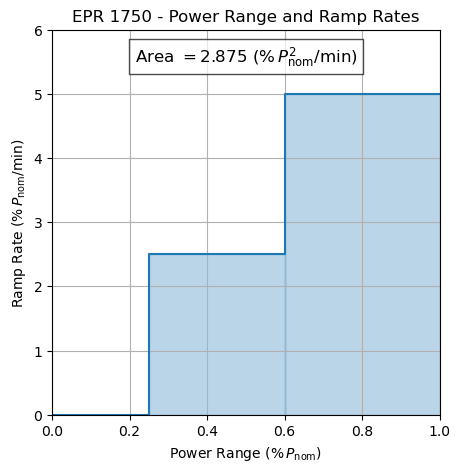
\includegraphics[width=0.7\textwidth]{imgs/load_following_curve.png}
    \caption{Example \gls{lfc} curve for EPR-1750}
    \label{fig:load-following-curve}
\end{figure}

\begin{table}[!hb]
    \centering
    \begin{tabularx}{\textwidth}{l X X}
        \toprule
        \textbf{Reactor Model} & \textbf{\gls{lfc} $\left[ \frac{\%P_{nom}^2}{min} \right]$} & Data Source \\
        \midrule
        APR1400         & 0.21  & \cite{iaea2025aris} \\
        EPR 1750        & 2.88 & \cite{OECD_NEA_Load_Following_2011} \\
        AP1000          & 4.25  & \cite{iaea2025aris} \\
        BWRX-300        & 0.25  & \cite{iaea2025aris} \\
        Rolls Royce SMR & 2.00 & \cite{iaea2025aris} \\
        NuScale         & 2.00   & \cite{ENCO_SMR_Analysis_2022} \\
        GE 9HA.02 2xCC & 7.02 & \cite{GE_9HA_Gas_Turbine_2015} \\
        GE LM2500XPRESS+G5 2xCC & 40.54 & \cite{GEVernova_LM2500XPRESS_2025} \\
        Hydroelectric   & >100 & \cite{OTA_Electric_Power_Wheeling_1989, osti_219975, MWH_Pumped_Storage_Wind_2009} \\
        \bottomrule
    \end{tabularx}
    \caption{Load following capabilities and power output}
    \label{tab:load-following-capabilities}
\end{table}

\subsection{Economic Indicators}

\paragraph{Capital Costs} are capital costs...

\begin{table}[!hb]
    \centering
    \begin{tabularx}{\textwidth}{X X X}
        \toprule
        \textbf{Option} & \textbf{PROs} & \textbf{CONs}\\
        \midrule
        Use NOAK estimates          & Use of estimates in all cases, comparable values & It's not realistic and not fair towards more mature designs \\
        \cmidrule(lr){1-3}
        Use FOAK estimates/data        & Better data for three large reactors & We are mixing up real data and estimates \\
        \cmidrule(lr){1-3}
        Use NOAK and apply FOAK-to-NOAK conversion         & Comparable values, with awareness of current know-how & rely on a model \\
        \cmidrule(lr){1-3}
        Present NOAK and FOAK to experts along with technological readiness overview and let them evaluate &  As before & rely on expert judgment \\
        \bottomrule
    \end{tabularx}
    \caption{Options overview}
    % \label{tab:operational-costs}
\end{table}

The same applies to commissioning time.

It is important to note that these costs refer to an Nth of a kind installation and will not be representative of the FOAK costs. Moreover as detailed by Rothwell 2022 \cite{ROTHWELL2022112905} the costs of recent nuclear installations in Europe and the US have been significantly higher than those announced at the start of the project. For this reason we will apply a FOAK-to-NOAK factor to better represent the real costs. For example the EPR-1600 announced costs for Flamanville-3 was 1886 $USD_{2020}/kW_e$ but have risen to 8600 $USD_{2020}/kW_e$ \cite{NEA2020}. All Values are summarized in Table \ref{tab:capital-costs}. \\

For reference, the capital costs of the same plants as the previous section have been reported by the US Energy Information Administration \cite{EIA_Capital_Costs_AEO2024}.

We want to clarify that the data has all been converted to 2020 USD since the main source of data \cite{STEIGERWALD2023128204} and \cite{NEA2020} reports all costs in this currency and year. \\

\begin{table}[!hb]
    \centering
    \begin{tabularx}{\textwidth}{l X X X}
        \toprule
        \textbf{Reactor Model} & \textbf{Capital Cost of NOAK [\$/kWe]} & \textbf{Capital Cost of FOAK [\$/kWe]} & Data Source \\
        \midrule
        APR-1400         & 1828 & 2410 & \cite{STEIGERWALD2023128204, NEA2020} \\
        EPR-1750        & 2150 & 8600 & \cite{STEIGERWALD2023128204, NEA2020} \\
        AP-1000          & 2000 & 8600 & \cite{STEIGERWALD2023128204, NEA2020} \\
        BWRX-300        & 2318 & 3467 & \cite{ReutersEvents2018} \\
        Rolls Royce SMR & 6050 & 7408 & \cite{PowerTechnology2022} \\
        NuScale         & 2850 & 3600 & \cite{NuScale2020} \\
        \textbf{Other Power Plants} & & & \\
        Onshore Wind   & - & 1265 & \cite{EIA_Capital_Costs_AEO2024} \\
        Solar PV + Battery & - & 2175 & \cite{EIA_Capital_Costs_AEO2024} \\
        Hydroelectric  & - & 6007 & \cite{EIA_Capital_Costs_AEO2024} \\
        \bottomrule
    \end{tabularx}
    \caption{Capital costs for selected reactor models}
    \label{tab:capital-costs}
\end{table}

\paragraph{Commissioning Time} see observations in the previous section.

I would apply a +0.5 years to planned commissioning time on the APR and AP based on the planned commissioning time of the EPR that differs by 0.5 between UK and Chinese plannings. 

\begin{table}[!hb]
    \centering
    \begin{tabularx}{\textwidth}{l X X c}
        \toprule
        \textbf{Reactor Model} & \textbf{Planned Commissioning Time} & \textbf{Last unit Commissioning Time} & Data Source\\
        \midrule
        APR1400         & 5.0 in Korea & 10 and 8 in Korea & \cite{nea2020unlocking} \\
        EPR 1750        & 5.0 in Europe, 4.5 in China & 9 in Taishan, 17 in Flamanville and Olkiluoto & \cite{nea2020unlocking} \\
        AP1000          & 5.0 in USA & 9 in Sanmen, 10 and 11 at Vogtle & \cite{nea2020unlocking} \\
        BWRX-300        & 2 $\sim$ 3 & NA & \cite{GEVernova_Nuclear_2025} \\
        Rolls Royce SMR & 4.0 & NA & \cite{RollsRoyce_SMR_Approach_2025} \\
        NuScale         & 3.0 & NA & \cite{NuScale_Power_Module_2025} \\
        \bottomrule
    \end{tabularx}
    \caption{Technological readiness and planned commissioning time}
    \label{tab:tech-readiness}
\end{table}


\paragraph{Operational Costs} are costs due to operations...

Steigerwald et al. (2023) \cite{STEIGERWALD2023128204} provides comprehensive cost analyses for future nuclear installations, including capital and operational expenditures for both SMRs and large reactors. The study reports operational costs in $USD_{2020}/MWh_e$ for EPR and APR1400 designs, as well as a "Long-Term US" category which this analysis uses as AP1000 costs. For SMRs, operational costs were originally presented in power-based units ($USD_{2020}/MW_e$), requiring conversion to energy-based measurements ($USD_{2020}/MWh_e$) using a Gaussian distribution of capacity factors ($\mu$ = 90\%, $\sigma$ = 5\%) according to:

$$
\frac{USD_{2020}}{MWh_e} = \frac{USD_{2020}}{MW_e} \cdot \frac{1}{CF \cdot 8760 \frac{h}{year}}
$$

The same study reports fuel costs of $6.23 USD_{2020}/MWh_e$ for PWR-based technologies with the exceptions of NuScale at $7.15 USD_{2020}/MWh_e$ and the only BWR reactor at $29.55 USD_{2020}/MWh_e$. For comparative context, operational cost estimates for utility-scale onshore wind, hydroelectric, and solar PV (with single axis tracking and DC battery storage) were obtained from the U.S. Energy Information Administration \cite{EIA_Capital_Costs_AEO2024}. All cost data have been standardized to 2020 USD to maintain consistency with the primary data sources \cite{STEIGERWALD2023128204, NEA2020}, values are presented in Table \ref{tab:operational-costs}.


\begin{table}[!hb]
    \centering
    \begin{tabularx}{\textwidth}{l X X}
        \toprule
        \textbf{Reactor Model} & \textbf{Operative Cost [\$/MWh]} & Data Source\\
        \midrule
        APR-1400          & 18.44 & \cite{STEIGERWALD2023128204} \\
        EPR-1750        & 14.26 & \cite{STEIGERWALD2023128204} \\
        AP-1000          & 18.69 & \cite{STEIGERWALD2023128204} \\
        BWRX-300        & $18.30 \pm 0.82$ & \cite{STEIGERWALD2023128204} \\
        Rolls Royce SMR & $65.68 \pm 2.94$ & \cite{STEIGERWALD2023128204} \\
        NuScale         & $22.76 \pm 1.02$ & \cite{STEIGERWALD2023128204} \\
        \textbf{Other Power Plants} & & \\
        Onshore Wind   & 28.08 & \cite{EIA_Capital_Costs_AEO2024} \\
        Solar PV + Battery & 33.33 & \cite{EIA_Capital_Costs_AEO2024} \\
        Hydroelectric  & 28.49 & \cite{EIA_Capital_Costs_AEO2024} \\
        \bottomrule
    \end{tabularx}
    \caption{Economic costs for selected reactor models}
    \label{tab:operational-costs}
\end{table}


\paragraph{Potential Impact on the energy market} can be estiated by...

\subsection{Indicators on Social Matters}
\paragraph{Potential Reduction of \glspl{ghg}} were quantified by comparing each country's 2024 emissions against projected emissions following deployment of one reactor unit. Country-specific GHG emission intensities were derived from Electricity Maps aggregated data \cite{ElectricityMaps_CarbonIntensity_2024}. Total load were obtained from the ENTSO-E Transparency Platform \cite{ENTSOE_Transparency_2025}. Due to non-normal data distributions, median values with interquartile ranges were employed to characterize uncertainty (Table~\ref{tab:ghg-intensity-country}). \\

\begin{table}[!ht]
    \centering
    \begin{tabularx}{\textwidth}{l c c c}
        \toprule
        Country / Region & Annual Load [TWh] & GHG intensity [gCO$_2$-eq/kWh] & Total annual GHG [MtCO$_2$-eq/yr] \\
        \midrule
        Italy (IT)        & draft & 240 & 72.0 \\
        Switzerland (CH)  & 60  & draft  & 1.8 \\
        Poland (PL)       & 160 & 700 & draft \\
        France (FR)       & 460 & draft  & 23.0 \\
        \bottomrule
    \end{tabularx}
    \caption{Country-level electricity load, grid GHG intensity and total annual GHG emissions. (Total = Load [TWh] * intensity [gCO$_2$-eq/kWh] / 1000)}
    \label{tab:ghg-intensity-country}
\end{table}

For nuclear generation's lifecycle emissions, Liu et al.'s (2023) comprehensive meta-analysis of 42 studies \cite{10.3389/fenrg.2023.1147016} served as the primary reference, reporting a global average of $15.815 \pm 3.59 \; gCO_{2,\text{eq}}/kWh_e$ for light water reactors. This conservative estimate was selected despite lower values observed in specific contexts: French nuclear operations typically range between $ 2 \sim 6 \; gCO_{2,\text{eq}}/kWh_e$ according to both operational data \cite{paillere_2021} and IAEA assessments \cite{IAEA_Climate_Change_Nuclear_Power_2022}, while individual studies on french reactors have reported values as high as $12 \; gCO_{2,\text{eq}}/kWh_e$ \cite{paillere_2021}. The global average was preferred to account for potential regional variations in fuel cycle practices and construction impacts. \\

Small modular reactors (SMRs) were assigned an emission intensity of $17.24 \pm 3.91$ $gCO_{2,\text{eq}}/kWh_e$, incorporating Carless et al.'s (2016) finding that SMRs exhibit approximately $9\%$ higher lifecycle emissions than conventional large LWRs due to reduced economies of scale in construction and fuel production \cite{CARLESS201684}. \\

The GHG reduction benefit was calculated as the percentage improvement between current energy mixes $GHG_{current\ mix}$  and the nuclear deployment scenario $GHG_{nuclear}$:
$$
GHG_{Benefit} (\%) = \left(1 - \frac{GHG_{nuclear}}{GHG_{current\ mix}}\right) \times 100
$$

% The results are shown in Table \ref{tab:ghg-benefit-country}.
% \begin{table}[!ht]
%     \centering
%     \begin{tabularx}{0.7\textwidth}{l c c}
%         \toprule
%         \textbf{Country/Region} & \textbf{GHG Reduction (Large) [tCO2/MWh]} & \textbf{GHG Reduction (SMR) [tCO2/MWh]} \\
%         \midrule
%         Italy (IT)        & 0.85 & 0.83 \\
%         Switzerland (CH)  & 0.10 & 0.09 \\
%         Poland (PO)       & 0.90 & 0.88 \\
%         France (FR)       & 0.15 & 0.14 \\
%         \bottomrule
%     \end{tabularx}
%     \caption{GHG emission intensity benefit by country for large reactors and SMRs}
%     \label{tab:ghg-benefit-country}
% \end{table}
\paragraph{Spent Nuclear Fuel Production} was estimated based on...

\paragraph{Mining Waste} are estimated ....

\paragraph{Percived Safety} is an important point ...


% Gathering data
\section{Data}
\label{sec:data}
\textcolor{orange}{This is a placeholder section, I'm writing down a description for each attribute and each data set that i used. I will then need to structure it properly to make it readable.}

\subsubsection{Thermal Efficiency}
Thermal efficiency indicates the fraction of thermal power generated by fission that is converted into net electrical power, accounting for in-plant consumption. Efficiency values were calculated using net electrical power output and thermal power data from the ARIS database \cite{iaea2025aris}:
$$
\eta = \frac{P_{el,net}}{P_{th}}
$$

\begin{table}[!ht]
    \centering
    \begin{tabularx}{\textwidth}{X c}
        \toprule
        \textbf{Reactor Model} & \textbf{Net Efficiency [\%]} \\
        \midrule
        APR1400         & 35.2 \\
        EPR 1750        & 36.2 \\
        AP1000          & 32.4 \\
        BWRX-300        & 34.5 \\
        Rolls Royce SMR & 34.6 \\
        NuScale         & 30.8 \\
        \bottomrule
    \end{tabularx}
    \caption{Net electrical efficiencies for selected reactor models}
    \label{tab:reactor-efficiency}
\end{table}



\subsubsection{Discharge Burnup}
Discharge burnup measures the energy extracted per unit of heavy metal fuel ($MWd/tonHM$). Data for APR1400 and AP1000 were sourced from the ARIS database \cite{iaea2025aris}, while EPR 1750 data were obtained from \cite{NRC_ML052280170}. Ranges are provided for SMRs due to design variability.

\begin{table}[!ht]
    \centering
    \begin{tabularx}{\textwidth}{X c}
        \toprule
        \textbf{Reactor Model} & \textbf{Discharge Burnup [$MWd/tonHM$]} \\
        \midrule
        APR1400         & 46.5 \\
        EPR 1750        & 55 \\
        AP1000          & 50 \\
        BWRX-300        & $50 \pm 5$ \\
        Rolls Royce SMR & $55 \pm 5$ \\
        NuScale         & $52.5 \pm 2.5$ \\
        \bottomrule
    \end{tabularx}
    \caption{Discharge burnup for selected reactor models}
    \label{tab:reactor-burnup}
\end{table}





\subsubsection{Technological Readiness and Planned Commissioning Time}
The technological Readiness Level is a purely qualitative score that is given on a scale from 1 to 13 as discrete values from the Fibonacci sequence (1,2,3,5,8,13), where 1 is the furtherst away from commercial deplyment and 13 is the closest to Nth-of-a-kind. The score considers the state of development, current number of units operational or under construction and licensing status as well as other considerations. The data was gathered from the ARIS database \cite{iaea2025aris} and from the respective company websites. \\

The APR1400 and the AP1000 are considered the most advanced reactors, with several units operational (9 and 7 respectively) and other under construction (3 and 2). The only catch with these designs is that none of these deployments has been made within Europe. On the other hand the EPR 1750 has only 2 operational units, both in China, 2 similar operational units (EPR 1650 in Olkiluoto and Flamanville) and 3 units Under construction in the UK (Hinkley Point and Sizewell). So these three reactors all get a 8/13 score, the first and the second don't get full points because of the lack of European experience, while the EPR 1750 doesn't get full points because of the limited number of operational units and the delays and overcosts that have plagued the first two EPRs. \\

Among the three SMRs the Rolls Royce SMR is the most similar to a conventional power plant being based on a multi-loop design with forced circulation, the know-how trasnferability for commissioing is considered high, as well as the managment of the construction site. For this it scores a 5/13. \\

The BWRX-300 is a more innovative design being an integrated reactor housing all the components of the NSSS within the reactor vessel, this means that the construction itself will be the first of his kind but this type of desing has been studied since 2010s \cite{PLACEHOLDER}. Moreover since the plan is to deploy just one unit the construction site will most likely be managed as a common nuclear power plant. For tthis it scores a 3/13. \\

At last, the Nuscale SMR has a compleltly novel design, not only is a natural circulation based, integrated PWR, but it is also ment to be deployed in a multi-unit configuration in a novel way. This means that the managment of the construction site itself will be new, for this it scores the lowest, a 2/13. \\



\begin{table}[!ht]
    \centering
    \begin{tabularx}{\textwidth}{l X X}
        \toprule
        \textbf{Reactor Model} & \textbf{Net Power Output $[MW_{e,net}]$} & Data Source\\
        \midrule
        APR1400         & 1340 & \cite{IAEA_PRIS_2025} \\
        EPR 1750        & 1630 & \cite{IAEA_PRIS_2025} \\
        AP1000          & 1120 & \cite{IAEA_PRIS_2025} \\
        BWRX-300        & 300 & \cite{iaea2025aris} \\
        Rolls Royce SMR & 470 & \cite{iaea2025aris} \\
        NuScale         & 77 (per unit) & \cite{iaea2025aris} \\
        \bottomrule
    \end{tabularx}
    \caption{Load following capabilities and power output}
    \label{tab:load-power_output}
\end{table}



\subsubsection{Radioactive Waste Produced}
TD

% Results are shown in Table \ref{tab:waste-produced}.
% \begin{table}[!ht]
%     \centering
%     \begin{tabularx}{0.6\textwidth}{l c}
%         \toprule
%         \textbf{Reactor Model} & \textbf{Waste Produced [kg/TWh]} \\
%         \midrule
%         APR1400         & 22 \\
%         EPR 1750        & 20 \\
%         AP1000          & 24 \\
%         BWRX-300        & 28 \\
%         Rolls Royce SMR & 30 \\
%         NuScale         & 35 \\
%         \bottomrule
%     \end{tabularx}
%     \caption{Radioactive waste produced per TWh}
%     \label{tab:waste-produced}
% \end{table}



\subsection{Country-Specific and Contextual Factors}
This subsection evaluates factors dependent on the deployment country, including fuel availability, regulatory environment, and supply chain adaptability.

\subsubsection{Fuel Manufacturing Feasibility by Country}
For this we have to consider two aspects, the first one is technolgy-wise and considers if the fuel exists or not. The second cosnideration is dependent on the coutry and considers if the that fuel is used in that country or how easy would it be to get to that country.

For the country aspect we can apply a correction factor as follows: 
$1$ is the fuel is already used in that country such as EPR fuel in France. $0.9$ if the fuel is used in other european countries since some paperwork will be needed but the open market will facilitate the import. $0.8$ for the same situation but for CH since the market has some barriers. $0.5$ is that fuel is not at all used in Europe and has to be imported from overseas.

Then regarding the tecnology, the 3 existing reactors get a 10/10 score, as well as the BWRX-300 since it will use an existing fuel assembly GNF-2 \cite{CNSC_BWRX300_Fuel_Design}. Rolls-Royce SMR and NuScale get a 5/10 since they will have to develop their own fuel but it will be a derivative of existing PWR fuel \cite{RollsRoyce_SMR_UK_Fuel_2023} and \cite{NRC_ML17007A001}. Rolls-Royce is working with Westinghouse for the fuel development \cite{PLACEHOLDER} while NuScale wants to modify the HTP\texttrademark{} fuel that is also produced by Framatome \cite{Framatome_GNF2_Fuel_2018}.

% So here there is a cross table with the reactors and the countries with the respective scores.

% \begin{table}[!ht]
%     \centering
%     \begin{tabularx}{0.9\textwidth}{l c c c c c}
%         \toprule
%         \textbf{Reactor Model} & \textbf{France (FR)} & \textbf{Switzerland (CH)} & \textbf{Poland (PO)} & \textbf{Northern Italy (NI)} & \textbf{Base Score} \\
%         \midrule
%         EPR1750         & 1.0 & 1.0 & 1.0 & 1.0 & 10 \\
%         APR1400         & 1.0 & 1.0 & 1.0 & 1.0 & 10 \\
%         AP1000          & 1.0 & 1.0 & 1.0 & 1.0 & 10 \\
%         BWRX-300        & 1.0 & 1.0 & 1.0 & 1.0 & 10 \\
%         Rolls Royce SMR & 1.0 & 1.0 & 1.0 & 1.0 & 5 \\
%         NuScale         & 1.0 & 1.0 & 1.0 & 1.0 & 5 \\
%         \bottomrule
%     \end{tabularx}
%     \caption{Fuel manufacturing feasibility scores by country}
%     \label{tab:fuel-feasibility}
% \end{table}



\subsubsection{Know-how Transferability and Supply Chain Adaptability}
Scores reflect the ease of transferring operational knowledge and adapting local supply chains. Know-how transferability considers the presence of similar designs in the country whereas supply chain adaptability considers the presence of the NSSS supplier in the country. For instance France has a lot of experience with PWR and has an EPR (of previous iteration at Flamanville) therefore will have a high know-how transferability for the EPR, on the other hand Italy has shut down all its reactors since 1986 therefore the know-how related score will be low for all reactors. Nonetheless Italy still has an active Nuclear Industry, with Ansaldo Nucleare operating in Genova and Framatome having offices in Milan. This means that even if the know-how is low, the supply chain can be esablished more easily. \\

The reason to separate these two aspects is to be able to give different importance (weights) to the human aspect (know-how) and the industrial/Economic aspect of the supply chain. \\

% The results are shown in Table \ref{tab:know-how-country} and Table \ref{tab:supply-chain-country}.

% \begin{table}[!ht]
%     \centering
%     \begin{minipage}{0.48\textwidth}
%         \centering
%         \begin{tabularx}{\textwidth}{l c c c c}
%             \toprule
%             \textbf{Reactor Model} & \textbf{IT} & \textbf{FR} & \textbf{CH} & \textbf{PO} \\
%             \midrule
%             APR1400         & 4 & 8 & 7 & 6 \\
%             EPR 1750        & 5 & 10 & 8 & 7 \\
%             AP1000          & 4 & 7 & 7 & 6 \\
%             BWRX-300        & 3 & 6 & 6 & 5 \\
%             Rolls Royce SMR & 3 & 6 & 5 & 5 \\
%             NuScale         & 2 & 5 & 4 & 4 \\
%             \bottomrule
%         \end{tabularx}
%         \caption{Know-how transferability scores by country}
%         \label{tab:know-how-country}
%     \end{minipage}
%     \hfill
%     \begin{minipage}{0.48\textwidth}
%         \centering
%         \begin{tabularx}{\textwidth}{l c c c c}
%             \toprule
%             \textbf{Reactor Model} & \textbf{IT} & \textbf{FR} & \textbf{CH} & \textbf{PO} \\
%             \midrule
%             APR1400         & 7 & 8 & 7 & 7 \\
%             EPR 1750        & 8 & 9 & 8 & 8 \\
%             AP1000          & 7 & 7 & 7 & 7 \\
%             BWRX-300        & 6 & 6 & 6 & 6 \\
%             Rolls Royce SMR & 6 & 7 & 6 & 6 \\
%             NuScale         & 5 & 6 & 5 & 5 \\
%             \bottomrule
%         \end{tabularx}
%         \caption{Supply chain adaptability scores by country}
%         \label{tab:supply-chain-country}
%     \end{minipage}
% \end{table}



\subsection{Economic and Political Indicators}
This subsection assesses macro-level indicators influencing project feasibility.


\subsubsection{Marginal Cost Impact}
TD

% Table \ref{tab:marginal-cost-impact} summarizes the qualitative impact.
% \begin{table}[!ht]
%     \centering
%     \begin{tabularx}{0.5\textwidth}{l c}
%         \toprule
%         \textbf{Reactor Model} & \textbf{Marginal Cost Impact} \\
%         \midrule
%         APR1400         & Low \\
%         EPR 1750        & Moderate \\
%         AP1000          & Low \\
%         BWRX-300        & High \\
%         Rolls Royce SMR & High \\
%         NuScale         & High \\
%         \bottomrule
%     \end{tabularx}
%     \caption{Marginal cost impact for selected reactor models}
%     \label{tab:marginal-cost-impact}
% \end{table}



\subsubsection{Country Economics and Politics}
These indicators are meant to represent a country's economic and political state. 
Real GDP from 2015 to 2030 (projected) and Expense as a percentage of GDP from 2015 to 2023 have been obtained from the International Monetary Fund \cite{PLACEHOLDER}. \\

Researchers in Research and Developments per million inhabitants from 2015 to 2023, as well as the GDP expenditure for Research have been obtained from the UNESCO Institute for Statistics \cite{PLACEHOLDER}. \\
Political Stability, a qualitative indicator ranging from $-2.5$ to $2.5$, has been obtained from the Worldwide Governance Indicators project by the World Bank \cite{PLACEHOLDER}. \\
Then from the V-Dem dataset \cite{PLACEHOLDER} we extracted:
\begin{itemize}
    \item v2x polyarchy: TO what extent is the people's opinion taken into account in the political process?
    \item v2regdur: Regime duration, how long has the last regime (goverment) lasted?
    \item v2cltrnslw: Are the laws and the political actions transparent, well publicized, coherent and stable thoughout the years?
    \item v2dlengage: To what extent are the citizens engaged in the political process?
\end{itemize}

Then we considered public support for nuclear energy, data was gathered from various sources \cite{PLACEHOLDER} \cite{PLACEHOLDER} \cite{PLACEHOLDER} \cite{PLACEHOLDER}.

The objective of these data is to create 2 contry-specific modifiers. One for their economic state, if a country is growing and tends to spend a lot in R\&D it will be more likely to be able to afford a nuclear project. The second indicator is to represent the support for nuclear energy, not only considering the current stance, but also trying to understand how stable this stance will be in the coming years.

% \begin{table}[!ht]
%     \centering
%     \begin{tabularx}{0.8\textwidth}{l c c c}
%         \toprule
%         \textbf{Country/Region} & \textbf{Real GDP Growth [\%]} & \textbf{Political Stability Score} & \textbf{Public Support for Nuclear [\%]} \\
%         \midrule
%         France          & 1.8 & 0.9 & 65 \\
%         Switzerland     & 1.2 & 0.8 & 45 \\
%         Poland          & 3.5 & 0.7 & 70 \\
%         Northern Italy  & 0.9 & 0.6 & 35 \\
%         \bottomrule
%     \end{tabularx}
%     \caption{Country economics and politics indicators}
%     \label{tab:country-indicators}
% \end{table}

\subsubsection{Electric data}
TD

\subsubsection{Environmental Impact: GHG Emission Intensity Benefit}

\subsubsection{GHG Emission Reduction Estimation}
Greenhouse gas (GHG) emission reductions were quantified by comparing each country's 2024 emissions against projected emissions following deployment of one reactor unit. Country-specific GHG emission intensities were derived from Electricity Maps \cite{ElectricityMaps_CarbonIntensity_2024}. Total load and cross-border flow measurements were obtained from the ENTSO-E Transparency Platform \cite{ENTSOE_Transparency_2025}. Due to non-normal data distributions, median values with interquartile ranges were employed to characterize uncertainty (Table~\ref{tab:ghg-intensity-country}). \\

For nuclear generation's lifecycle emissions, Liu et al.'s (2023) comprehensive meta-analysis of 42 studies \cite{10.3389/fenrg.2023.1147016} served as the primary reference, reporting a global average of $15.815 \pm 3.59 \; gCO_{2,\text{eq}}/kWh_e$ for light water reactors. This conservative estimate was selected despite lower values observed in specific contexts: French nuclear operations typically range between $ 2 \sim 6 \; gCO_{2,\text{eq}}/kWh_e$ according to both operational data \cite{paillere_2021} and IAEA assessments \cite{IAEA_Climate_Change_Nuclear_Power_2022}, while individual studies on french reactors have reported values as high as $12 \; gCO_{2,\text{eq}}/kWh_e$ \cite{paillere_2021}. The global average was preferred to account for potential regional variations in fuel cycle practices and construction impacts. \\

Small modular reactors (SMRs) were assigned an emission intensity of $17.24 \pm 3.91$ $gCO_{2,\text{eq}}/kWh_e$, incorporating Carless et al.'s (2016) finding that SMRs exhibit approximately $9\%$ higher lifecycle emissions than conventional large LWRs due to reduced economies of scale in construction and fuel production \cite{CARLESS201684}. \\

The GHG reduction benefit was calculated as the percentage improvement between current energy mixes $GHG_{current\ mix}$  and the nuclear deployment scenario $GHG_{nuclear}$:
$$
GHG_{Benefit} (\%) = \left(1 - \frac{GHG_{nuclear}}{GHG_{current\ mix}}\right) \times 100
$$

% The results are shown in Table \ref{tab:ghg-benefit-country}.
% \begin{table}[!ht]
%     \centering
%     \begin{tabularx}{0.7\textwidth}{l c c}
%         \toprule
%         \textbf{Country/Region} & \textbf{GHG Reduction (Large) [tCO2/MWh]} & \textbf{GHG Reduction (SMR) [tCO2/MWh]} \\
%         \midrule
%         Italy (IT)        & 0.85 & 0.83 \\
%         Switzerland (CH)  & 0.10 & 0.09 \\
%         Poland (PO)       & 0.90 & 0.88 \\
%         France (FR)       & 0.15 & 0.14 \\
%         \bottomrule
%     \end{tabularx}
%     \caption{GHG emission intensity benefit by country for large reactors and SMRs}
%     \label{tab:ghg-benefit-country}
% \end{table}



\subsubsection{Import Dependence}
TD

\subsubsection{Policy Stability and Long-Term Project Viability}







% Example citation to avoid compilation errors :D
\nocite{*}

% \printbibliography
\end{document}
